% GNUPLOT: LaTeX picture with Postscript
\begingroup
\newcommand\ft\footnotesize\newcommand\st\scriptsize
  \makeatletter
  \providecommand\color[2][]{%
    \GenericError{(gnuplot) \space\space\space\@spaces}{%
      Package color not loaded in conjunction with
      terminal option `colourtext'%
    }{See the gnuplot documentation for explanation.%
    }{Either use 'blacktext' in gnuplot or load the package
      color.sty in LaTeX.}%
    \renewcommand\color[2][]{}%
  }%
  \providecommand\includegraphics[2][]{%
    \GenericError{(gnuplot) \space\space\space\@spaces}{%
      Package graphicx or graphics not loaded%
    }{See the gnuplot documentation for explanation.%
    }{The gnuplot epslatex terminal needs graphicx.sty or graphics.sty.}%
    \renewcommand\includegraphics[2][]{}%
  }%
  \providecommand\rotatebox[2]{#2}%
  \@ifundefined{ifGPcolor}{%
    \newif\ifGPcolor
    \GPcolortrue
  }{}%
  \@ifundefined{ifGPblacktext}{%
    \newif\ifGPblacktext
    \GPblacktextfalse
  }{}%
  % define a \g@addto@macro without @ in the name:
  \let\gplgaddtomacro\g@addto@macro
  % define empty templates for all commands taking text:
  \gdef\gplbacktext{}%
  \gdef\gplfronttext{}%
  \makeatother
  \ifGPblacktext
    % no textcolor at all
    \def\colorrgb#1{}%
    \def\colorgray#1{}%
  \else
    % gray or color?
    \ifGPcolor
      \def\colorrgb#1{\color[rgb]{#1}}%
      \def\colorgray#1{\color[gray]{#1}}%
      \expandafter\def\csname LTw\endcsname{\color{white}}%
      \expandafter\def\csname LTb\endcsname{\color{black}}%
      \expandafter\def\csname LTa\endcsname{\color{black}}%
      \expandafter\def\csname LT0\endcsname{\color[rgb]{1,0,0}}%
      \expandafter\def\csname LT1\endcsname{\color[rgb]{0,1,0}}%
      \expandafter\def\csname LT2\endcsname{\color[rgb]{0,0,1}}%
      \expandafter\def\csname LT3\endcsname{\color[rgb]{1,0,1}}%
      \expandafter\def\csname LT4\endcsname{\color[rgb]{0,1,1}}%
      \expandafter\def\csname LT5\endcsname{\color[rgb]{1,1,0}}%
      \expandafter\def\csname LT6\endcsname{\color[rgb]{0,0,0}}%
      \expandafter\def\csname LT7\endcsname{\color[rgb]{1,0.3,0}}%
      \expandafter\def\csname LT8\endcsname{\color[rgb]{0.5,0.5,0.5}}%
    \else
      % gray
      \def\colorrgb#1{\color{black}}%
      \def\colorgray#1{\color[gray]{#1}}%
      \expandafter\def\csname LTw\endcsname{\color{white}}%
      \expandafter\def\csname LTb\endcsname{\color{black}}%
      \expandafter\def\csname LTa\endcsname{\color{black}}%
      \expandafter\def\csname LT0\endcsname{\color{black}}%
      \expandafter\def\csname LT1\endcsname{\color{black}}%
      \expandafter\def\csname LT2\endcsname{\color{black}}%
      \expandafter\def\csname LT3\endcsname{\color{black}}%
      \expandafter\def\csname LT4\endcsname{\color{black}}%
      \expandafter\def\csname LT5\endcsname{\color{black}}%
      \expandafter\def\csname LT6\endcsname{\color{black}}%
      \expandafter\def\csname LT7\endcsname{\color{black}}%
      \expandafter\def\csname LT8\endcsname{\color{black}}%
    \fi
  \fi
    \setlength{\unitlength}{0.0500bp}%
    \ifx\gptboxheight\undefined%
      \newlength{\gptboxheight}%
      \newlength{\gptboxwidth}%
      \newsavebox{\gptboxtext}%
    \fi%
    \setlength{\fboxrule}{0.5pt}%
    \setlength{\fboxsep}{1pt}%
\begin{picture}(4932.00,5102.00)%
    \gplgaddtomacro\gplbacktext{%
      \colorrgb{0.50,0.50,0.50}%
      \put(478,4861){\makebox(0,0)[r]{\strut{}\ft $2$}}%
      \colorrgb{0.50,0.50,0.50}%
      \put(478,4171){\makebox(0,0)[r]{\strut{}\ft $1$}}%
      \colorrgb{0.50,0.50,0.50}%
      \put(478,3480){\makebox(0,0)[r]{\strut{}\footnotesize $0$}}%
      \colorrgb{0.50,0.50,0.50}%
      \put(478,2790){\makebox(0,0)[r]{\strut{}\ft $-1$}}%
      \colorrgb{0.50,0.50,0.50}%
      \put(936,2633){\makebox(0,0){\strut{}}}%
      \colorrgb{0.50,0.50,0.50}%
      \put(1627,2633){\makebox(0,0){\strut{}}}%
      \colorrgb{0.50,0.50,0.50}%
      \put(2317,2633){\makebox(0,0){\strut{}}}%
    }%
    \gplgaddtomacro\gplfronttext{%
      \csname LTb\endcsname%
      \put(170,3825){\rotatebox{-270}{\makebox(0,0){\strut{}$y$ / m}}}%
      \put(1626,2457){\makebox(0,0){\strut{}}}%
      \csname LTb\endcsname%
      \put(1627,4965){\makebox(0,0){\strut{}\ft $\sfpressure[superscript=sampled](\sfx,\sfy,\sfomega)$}}%
    }%
    \gplgaddtomacro\gplbacktext{%
      \colorrgb{0.50,0.50,0.50}%
      \put(2698,4861){\makebox(0,0)[r]{\strut{}}}%
      \colorrgb{0.50,0.50,0.50}%
      \put(2698,4171){\makebox(0,0)[r]{\strut{}}}%
      \colorrgb{0.50,0.50,0.50}%
      \put(2698,3480){\makebox(0,0)[r]{\strut{}}}%
      \colorrgb{0.50,0.50,0.50}%
      \put(2698,2790){\makebox(0,0)[r]{\strut{}}}%
      \colorrgb{0.50,0.50,0.50}%
      \put(3156,2633){\makebox(0,0){\strut{}}}%
      \colorrgb{0.50,0.50,0.50}%
      \put(3846,2633){\makebox(0,0){\strut{}}}%
      \colorrgb{0.50,0.50,0.50}%
      \put(4536,2633){\makebox(0,0){\strut{}}}%
    }%
    \gplgaddtomacro\gplfronttext{%
      \csname LTb\endcsname%
      \put(3138,3825){\rotatebox{-270}{\makebox(0,0){\strut{}}}}%
      \put(3846,2457){\makebox(0,0){\strut{}}}%
      \csname LTb\endcsname%
      \put(3846,4965){\makebox(0,0){\strut{}\ft $\sfpressure[superscript=sampled]_0(\sfx,\sfy,\sfomega) = \sfpressure(\sfx,\sfy,\sfomega)$}}%
    }%
    \gplgaddtomacro\gplbacktext{%
      \colorrgb{0.50,0.50,0.50}%
      \put(478,2515){\makebox(0,0)[r]{\strut{}\ft $2$}}%
      \colorrgb{0.50,0.50,0.50}%
      \put(478,1824){\makebox(0,0)[r]{\strut{}\ft $1$}}%
      \colorrgb{0.50,0.50,0.50}%
      \put(478,1134){\makebox(0,0)[r]{\strut{}\footnotesize $0$}}%
      \colorrgb{0.50,0.50,0.50}%
      \put(478,443){\makebox(0,0)[r]{\strut{}\ft $-1$}}%
      \colorrgb{0.50,0.50,0.50}%
      \put(936,286){\makebox(0,0){\strut{}\footnotesize $-1$}}%
      \colorrgb{0.50,0.50,0.50}%
      \put(1627,286){\makebox(0,0){\strut{}\footnotesize $0$}}%
      \colorrgb{0.50,0.50,0.50}%
      \put(2317,286){\makebox(0,0){\strut{}\footnotesize $1$}}%
    }%
    \gplgaddtomacro\gplfronttext{%
      \csname LTb\endcsname%
      \put(170,1479){\rotatebox{-270}{\makebox(0,0){\strut{}$y$ / m}}}%
      \put(1626,66){\makebox(0,0){\strut{}$x$ / m}}%
      \csname LTb\endcsname%
      \put(1627,2619){\makebox(0,0){\strut{}\ft $\sfpressure[superscript=sampled]_1(\sfx,\sfy,\sfomega) = \sfpressure[superscript=sampled]_{-1}(-\sfx,\sfy,\sfomega)$}}%
    }%
    \gplgaddtomacro\gplbacktext{%
      \colorrgb{0.50,0.50,0.50}%
      \put(2698,2514){\makebox(0,0)[r]{\strut{}}}%
      \colorrgb{0.50,0.50,0.50}%
      \put(2698,1824){\makebox(0,0)[r]{\strut{}}}%
      \colorrgb{0.50,0.50,0.50}%
      \put(2698,1134){\makebox(0,0)[r]{\strut{}}}%
      \colorrgb{0.50,0.50,0.50}%
      \put(2698,444){\makebox(0,0)[r]{\strut{}}}%
      \colorrgb{0.50,0.50,0.50}%
      \put(3156,287){\makebox(0,0){\strut{}\footnotesize $-1$}}%
      \colorrgb{0.50,0.50,0.50}%
      \put(3846,287){\makebox(0,0){\strut{}\footnotesize $0$}}%
      \colorrgb{0.50,0.50,0.50}%
      \put(4536,287){\makebox(0,0){\strut{}\footnotesize $1$}}%
    }%
    \gplgaddtomacro\gplfronttext{%
      \csname LTb\endcsname%
      \put(3138,1479){\rotatebox{-270}{\makebox(0,0){\strut{}}}}%
      \put(3846,67){\makebox(0,0){\strut{}$x$ / m}}%
      \csname LTb\endcsname%
      \put(3846,2618){\makebox(0,0){\strut{}\ft $\sfpressure[superscript=sampled]_2(\sfx,\sfy,\sfomega) = \sfpressure[superscript=sampled]_{-2}(-\sfx,\sfy,\sfomega)$}}%
    }%
    \gplbacktext
    \put(0,0){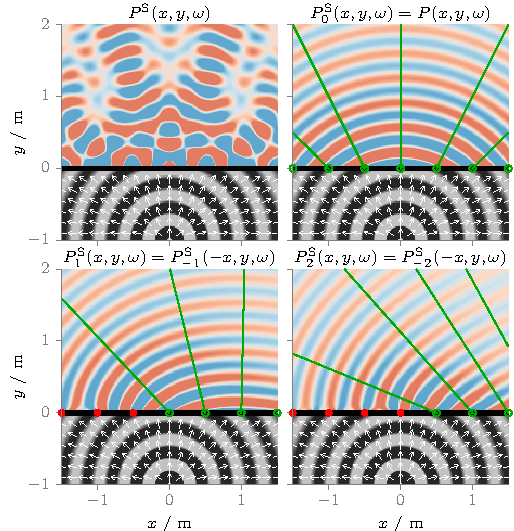
\includegraphics{fig}}%
    \gplfronttext
  \end{picture}%
\endgroup
